% !TeX root = Tesis.tex
% !TeX encoding = UTF-8
% !TeX spellcheck = es_ES
\chapter*{Introducción} \label{intro}
\addcontentsline{toc}{chapter}{Introducción}
\onehalfspacing

El \textit{fitness} celular refiere a la capacidad de una célula de sobrevivir y proliferar en un ambiente determinado. Abarca varios factores como la capacidad de la célula para adaptarse al ambiente, resistir al estrés y mantener la homeostasis. Este concepto es particularmente importante en la biología del cáncer, donde los niveles de \textit{fitness} celular pueden determinar su supervivencia y dominancia dentro de un tejido.

Un paradigma conocido en la biología molecular expresa que los máximos locales de \textit{fitness}, en el espacio de expresión genética, están relacionados con estados biológicos accesibles. Un diagrama de Wright es una representación gráfica reducida del panorama genético, donde los picos y valles representan diferentes genotipos y sus niveles relativos de \textit{fitness} \cite{wright1932roles}, ver Fig. \ref{fig:wrightDiagram}. 

\begin{figure}[!htb]
	\centering
	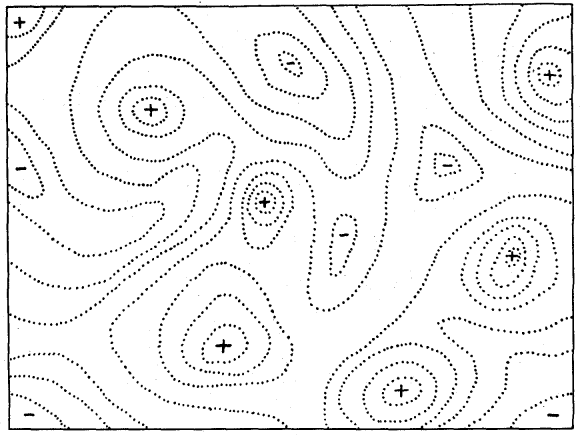
\includegraphics[scale=0.645]{figures/wright_diagram.png}
	\caption{Representación esquemática de un diagrama de Wright. Las zonas de mayor \textit{fitness} (+) están asociadas con estados biológicos accesibles. Las de menor \textit{fitness} (-) son solo zonas de transito. Las lineas discontinuas delimitan los distintos niveles de \textit{fitness}. Tomada de la referencia \cite{wright1932roles}.}
	\label{fig:wrightDiagram}
\end{figure}

Esta representación ha sido aplicada a la descripción del destino celular a lo largo de una línea de diferenciación \cite{casey2020theory}. Sin embargo, hasta donde sabemos, no hay gráficos basados en datos reales para un tejido dado que represente, al menos de forma parcial, un diagrama de Wright con más de dos máximos. En el presente trabajo, mostramos un diagrama para la materia blanca del cerebro en el cual el estado normal (N) se representa junto con el atractor glioblastoma (GB) y el máximo relacionado con la enfermedad del Alzheimer (EA).

La EA se caracteriza por la pérdida progresiva de células neuronales, mientras que el GB es un tipo de cáncer cerebral que implica la proliferación descontrolada de células. Algunas investigaciones muestran que pacientes con la EA podrían tener un menor riesgo de desarrollar GB. Por ejemplo, en la referencia \cite{ou2012does} se muestra que ambas enfermedades presentan un aumento en el estrés oxidativo, en la EA, esto hace que las células neuronales sean más vulnerables a la muerte, mientras que en el GB, las células cancerosas se vuelven más resistentes. Además, se plantea que la degeneración de células que secretan acetilcolina en la EA podría tener un efecto protector contra el cáncer, ya que esta sustancia puede estimular el crecimiento de células cancerosas.


%En \cite{Driver_2012} concluyen que los sobrevivientes de cáncer tienen un riesgo 33 \% menor de desarrollar la EA en comparación con aquellos sin antecedentes de cáncer. Las personas con la EA tienen un riesgo 61 \% menor de desarrollar cáncer. En \cite{Musicco_2013} encuentran que el riesgo de cáncer en pacientes con la EA se reduce a la mitad, y el riesgo de padecer la EA en pacientes con cáncer se reduce en un 35 \%.
Los estudios epidemiológicos señalan que aquellas personas que padecen una de estas enfermedades tiene un riesgo menor de desarrollar la otra. Concretamente, los pacientes con cáncer tienen un riesgo alrededor de 31 y 35 \% menor de desarrollar la EA en comparación con aquellos sin antecedente de cáncer. Mientras que las personas que padecen la EA tienen un riesgo entre 41 y 61 \% menor de desarrollar cáncer \cite{Roe_2010, Driver_2012, Musicco_2013}.
%Como se reporta en  \cite{Roe_2010, Driver_2012, Musicco_2013}, los datos sugieren que los pacientes con cáncer tienen un riesgo alrededor de 31 y 35 \% menor de desarrollar la EA en comparación con aquellos sin antecedente de cáncer. Mientras que los personas que padecen la EA tienen un riesgo entre 41 y 61 \% menor de desarrollar cáncer.

Esta idea de la EA y el GB como alternativas opuestas también está apoyada por un gran número experimentos de biología molecular. Por ejemplo, en la referencia \cite{Liu_2013} los autores encuentran que las vías de señalización ERK/MAPK están aumentadas en GB y disminuidas en la EA. Estas vías conectan señales extracelulares, como factores de crecimiento y citocinas, a respuestas intracelulares que regulan la proliferación celular, diferenciación y supervivencia. También muestran que las vías de señalización de la angiopoyetina están aumentadas en la EA y disminuidas en GB, estas relacionadas con la regulación de la angiogénesis y la estabilidad vascular.

El estudio realizados por C. Lanni y colaboradores en la referencia \cite{Lanni_2020} destaca varios actores moleculares, especialmente PIN1 y p53, que están involucrados en interacciones moleculares complejas asociadas con la correlación inversa entre estas enfermedades. El aumento en la expresión de PIN1 esta relacionado con un retraso en la edad de inicio de la EA, mientras niveles bajos de expresión se asocian con un menor riesgo de desarrollar varios tipos de cáncer.

% TODO: Tal vez pueda hablar un poco más del proceso de envejecimiento y de la teoría del envejecimiento programado
Muchas de estas investigaciones no solo muestran una oposición entre la EA y el GB, sino que también señalan el envejecimiento como un factor de riesgo común para ambas enfermedades \cite{Driver_2012, Musicco_2013 , Liu_2013, Lanni_2020, A_Driver_2010}. Esta compleja relación entre ambas enfermedades cerebrales queda representada en nuestro diagrama de Wright. Además, se puede apreciar un camino o corredor hacia el envejecimiento normal, en línea con la teoría del envejecimiento programado \cite{Magalh_es_2012, 	Gems_2022}.

A nivel genético, hay genes que varían su expresión de la misma manera en los procesos de envejecimiento, progresión al cáncer y la EA, mientras que también hay genes que indican una situación disyuntiva entre la EA y el GB. Un ejemplo de este último es el gen codificador de proteínas MMP9, que juega un papel importante en la invasión tumoral \cite{Choe2002, Xue_2017}, pero también conocido como neuroprotector, controlando las interacciones entre axones y fibras beta-amiloide \cite{Kaminari_2017}. Las desviaciones del valor de expresión genética de su referencia en el tejido normal pueden indicar una progresión potencial a la EA (subexpresión) o al GB (sobreexpresión).

Esta visión inusual puede ayudar a comprender las relaciones entre la EA y el GB, e identificar marcadores génicos útiles para ambos procesos. Como un bono adicional, la representación permite encontrar preguntas muy interesantes que se discutirán a continuación.

El trabajo presentado como tesis de maestría consta de una introducción, tres capítulos, las conclusiones y las recomendaciones. El contenido se distribuye de la siguiente forma:

\begin{itemize}
	\item[$\bullet$] \textbf{Introducción:} Se presenta análisis del panorama genético y epidemiológico relacionado con la EA, el GB y el envejecimiento. Se describe la relación inversa entre la EA y el GB basada en evidencia epidemiológica y molecular. Además, se hace referencia a la idea del envejecimiento programado como factor de riesgo para ambas enfermedades.
	
	\item[$\bullet$] \textbf{Capítulo 1:} Se centra en los métodos y materiales utilizados para analizar los datos de expresión genética. Se detalla la aplicación de técnicas de reducción de dimensionalidad, para simplificar y visualizar conjuntos de datos complejos. Además, se describen las dos principales fuentes de datos. Se explica también el procesamiento de los datos y su conversión a una expresión diferencial logarítmica para facilitar el análisis comparativo.
	
	\item[$\bullet$] \textbf{Capítulo 2:} Se centra en la construcción y análisis del diagrama de tres atractores que emergen en el espacio de expresión genética. Mediante técnicas de reducción dimensional se visualizan las posiciones relativas de estos atractores y se observa cómo las muestras de tejido se desplazan de un estado a otro. Además, se introduce un panorama del fitness celular a través de un diagrama de Wright que ilustra las barreras y la fuerza relativa de cada atractor, enfatizando las diferencias en la transición de un estado a otro.
	
	\item[$\bullet$] \textbf{Capítulo 3:} Presenta los resultados obtenidos del análisis de los datos de expresión genética. En este capítulo se destacan, por un lado, los hallazgos cualitativos, en los que se identifican claramente los atractores asociados al estado normal, al glioblastoma y a la enfermedad de Alzheimer, evidenciando las trayectorias y transiciones entre estos estados; y, por otro lado, se ofrece una perspectiva cuantitativa, respaldada por representaciones gráficas y análisis estadísticos, que valida la relación inversa entre el glioblastoma y el Alzheimer y resalta el papel del envejecimiento en estas transiciones.
	
	\item[$\bullet$] \textbf{Conclusiones:} Se sintetiza como el análisis de la expresión génica en la materia blanca del cerebro permite identificar tres atractores y ponen de manifiesto una relación inversa entre el desarrollo del glioblastoma y la aparición del Alzheimer. 
	
	\item[$\bullet$] \textbf{Recomendaciones:} Se destaca la necesidad de realizar estudios futuros que afinen y amplíen el modelo propuesto, proponiendo la integración de técnicas analíticas más robustas y la incorporación de datos de plataforma unificada para superar las limitaciones actuales de heterogeneidad.
	
	
\end{itemize}